% !TEX root = main.tex

\section{模态逻辑}
\begin{definition}[模态逻辑(modal logic)]
BNF定义如下
\[\phi::=\top\mid
\bot\mid
p\mid
(\lnot\phi)\mid
(\phi\land\phi)\mid
(\phi\lor\phi)\mid
(\phi\to\phi)\mid
(\phi\leftrightarrow\phi)\mid
(\square\phi)\mid
(\Diamond\phi)\]
其中$\square$为一定(necessarily),$\Diamond$为可能(possibly)。
优先级顺序
\begin{itemize}
	\item $\lnot,\square,\Diamond$
	\item $\lor,\land$
	\item $\to,\leftrightarrow$
\end{itemize}
\end{definition}
\begin{definition}[模型(model)]
模态逻辑的模型$\mM$由以下三个成分定义:
\begin{itemize}
	\item 世界(world)元素$W$
	\item 定义在$W$上的可访问(accessibility)关系$R\subset W\times W$
	\item 标记函数(labeling)$L:W\to\mathcal{P}(Atoms)$
\end{itemize}
这些模型称为Kripke模型
\end{definition}
\begin{figure}[H]
\centering
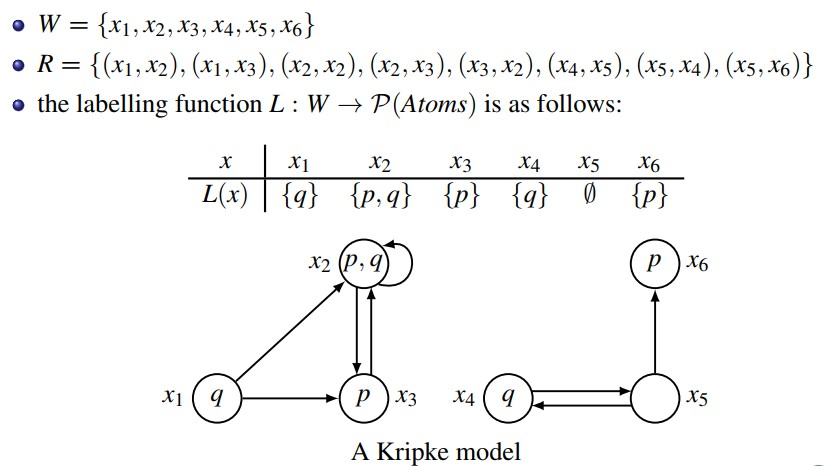
\includegraphics[width=0.8\linewidth]{fig/kripke_model.jpg}
\end{figure}

\begin{definition}
令$\mM=(W,R,L)$为基本的模态逻辑,$x\in W$和$\phi$是公式,满足性(satisfaction)关系$x\Vdash\phi$为在$\phi$上的结构推断(structural induction):
\[\begin{array}{rll}
x & \Vdash\top\\
x & \not\Vdash\bot\\
x & \Vdash p & \text{iff } p\in L(x)\\
x & \Vdash\lnot\phi & \text{iff } x\not\Vdash\phi\\
x & \Vdash\phi\land\psi & \text{iff } x\Vdash\phi \text{ and } x\Vdash\psi\\
x & \Vdash\phi\lor\psi & \text{iff } x\Vdash\phi \text{ or } x\Vdash\psi\\
x & \Vdash\phi\to\psi & \text{iff } x\Vdash\psi \text{ whenever } x\Vdash\phi\\
x & \Vdash\phi\leftrightarrow\psi & \text{iff } (x\Vdash\phi \text{ iff } x\Vdash\psi)\\
x & \Vdash\square\psi & \text{iff }\forall y\in W, R(x,y):\; y\Vdash\psi\\
x & \Vdash\Diamond\psi & \text{iff }\exists y\in W, R(x,y):\; y\Vdash\psi
\end{array}\]
\end{definition}
\begin{example}
比如上图的例子有
\begin{itemize}
	\item $x_1\Vdash q$,因$q\in L(x_1)$
	\item $x_1\Vdash\Diamond q$,因$R(x_1)=\{x_2,x_3\},x_2\in R(x_1),q\in L(x_2)$
	\item $x_1\not\Vdash\square q$,因$R(x_1)=\{x_2,x_3\},x_3\in R(x_1),q\notin L(x_3)$
\end{itemize}
\end{example}

De Morgan定律
\[\lnot\square\phi\equiv\Diamond\lnot\phi\qquad
\lnot\Diamond\phi\equiv\square\lnot\phi\]
分配律
\[\square(\phi\land\psi)\equiv\square\phi\land\square\psi\qquad
\Diamond(\phi\lor\psi)\equiv\Diamond\phi\lor\Diamond\psi\]
K模式(scheme)
\[\square(\phi\to\psi)\land\square\phi\to\square\psi\]
\begin{example}
证明$\lnot\square\phi\equiv\Diamond\lnot\phi$
\end{example}
\begin{analysis}
假设$x$是模型$\mM=(W,R,L)$的一个世界,希望找到$x\Vdash\lnot\square\phi\leftrightarrow\Diamond\lnot\phi$
\[\begin{aligned}
& x\Vdash\lnot\square\phi\\
\leftrightarrow & \text{it is not the case that } x\Vdash\square\phi\\
\leftrightarrow & \text{it is not the case that } \forall y\in R(x), y\Vdash\phi\\
\leftrightarrow & \exists y\in R(x)\text{ and not }y\Vdash\phi\\
\leftrightarrow & \exists y\in R(x)\text{ and }y\Vdash\lnot\phi\\
\leftrightarrow & x\Vdash\Diamond\lnot\phi
\end{aligned}\]
\end{analysis}